\documentclass[11pt]{beamer}
\usetheme{PaloAlto}
\usecolortheme{spruce}
\usepackage[spanish]{babel}
\usefonttheme{professionalfonts}
\usefonttheme{serif}
\usepackage{minted}
\usepackage{fontspec}
\setmainfont{Liberation Serif}
\usepackage{amsmath}
\usepackage{amsfonts}
\usepackage{amssymb}
\usepackage{graphicx}
\usepackage{menukeys} 
%Se configura minted
\definecolor{bg}{rgb}{0.95,0.95,0.95}
%\newminted{python}{fontsize=\scriptsize, 
%		   linenos,
%		   numbersep=8pt,
%		   gobble=4,
%		   frame=lines,
%		   bgcolor=bg,
%		   framesep=3mm} 
%\newminted{pycon}{bgcolor=bg, linenos=true, tabsize=4}
%\newcommand{\tab}[1][1cm]{\hspace*{#1}}

\author{Nelson David Pérez Garecía\\}
\title{Introducción a SEISAN:\\Sesión I}
%\setbeamercovered{transparent} 
%\setbeamertemplate{navigation symbols}{} 
%\logo{} 
\institute{Red Sismológica Nacional, \\Servicio Geológico Colombiano} 
\date{} 
%\subject{} 
\begin{document}

\begin{frame}
\titlepage
\begin{center}
\begin{figure}

\includegraphics[scale=0.15]{Logo-SGC.jpg}
\end{figure}
\end{center}
\end{frame}

\begin{frame}
\tableofcontents
\end{frame}

\section{Introducción}
\subsection{Prerrequisitos}
\begin{frame}{Prerrequisitos}
Para el uso de SEISAN es aconsejable tener conocimiento mínimo en los siguientes temas:
\begin{itemize}
\item Sismología de terremotos.
\pause
\item Sitema operativo UNIX/LINUX. 
\end{itemize}
\end{frame}

\begin{frame}{Prerrequisitos (Linux)}
Algunos comandos básicos de Linux:
\begin{table}
{\small
\begin{tabular}{|c|c|c|}
\hline 
 {\bf Comando} & {\bf Descripción} & {\bf Ejemplos}\\ 
\hline 
cat  & Concatena y muestra un archivo & cat /etc/passwd\\ 
\hline 
ls & Lista los archivos del directorio & ls /bd/seismo \\ 
\hline 
cd & Cambia el directorio & cd /tmp \\ 
\hline 
cp & Copia archivos & cp foo foo.backup \\ 
\hline 
mkdir & Crea un directorio & mkdir seismo \\ 
\hline 
mv & Mueve un archivo a un directorio & mv a.out prog1 \\ 
\hline 
more/less & Visualiza página a página un archivo & more foo.txt \\ 
\hline 
rm  & Borra un archivo & rm foo.c \\ 
\hline 
rm -r  & Borra un directorio & rm -r /bd/seismo\\ 
\hline 
pwd & Muestra la ruta del directorio actual & pwd \\ 
\hline
\end{tabular}}
\end{table} 
\end{frame}
\subsection{¿Qué es SEISAN?}
\begin{frame}{¿Qué es SEISAN?}
\begin{figure}
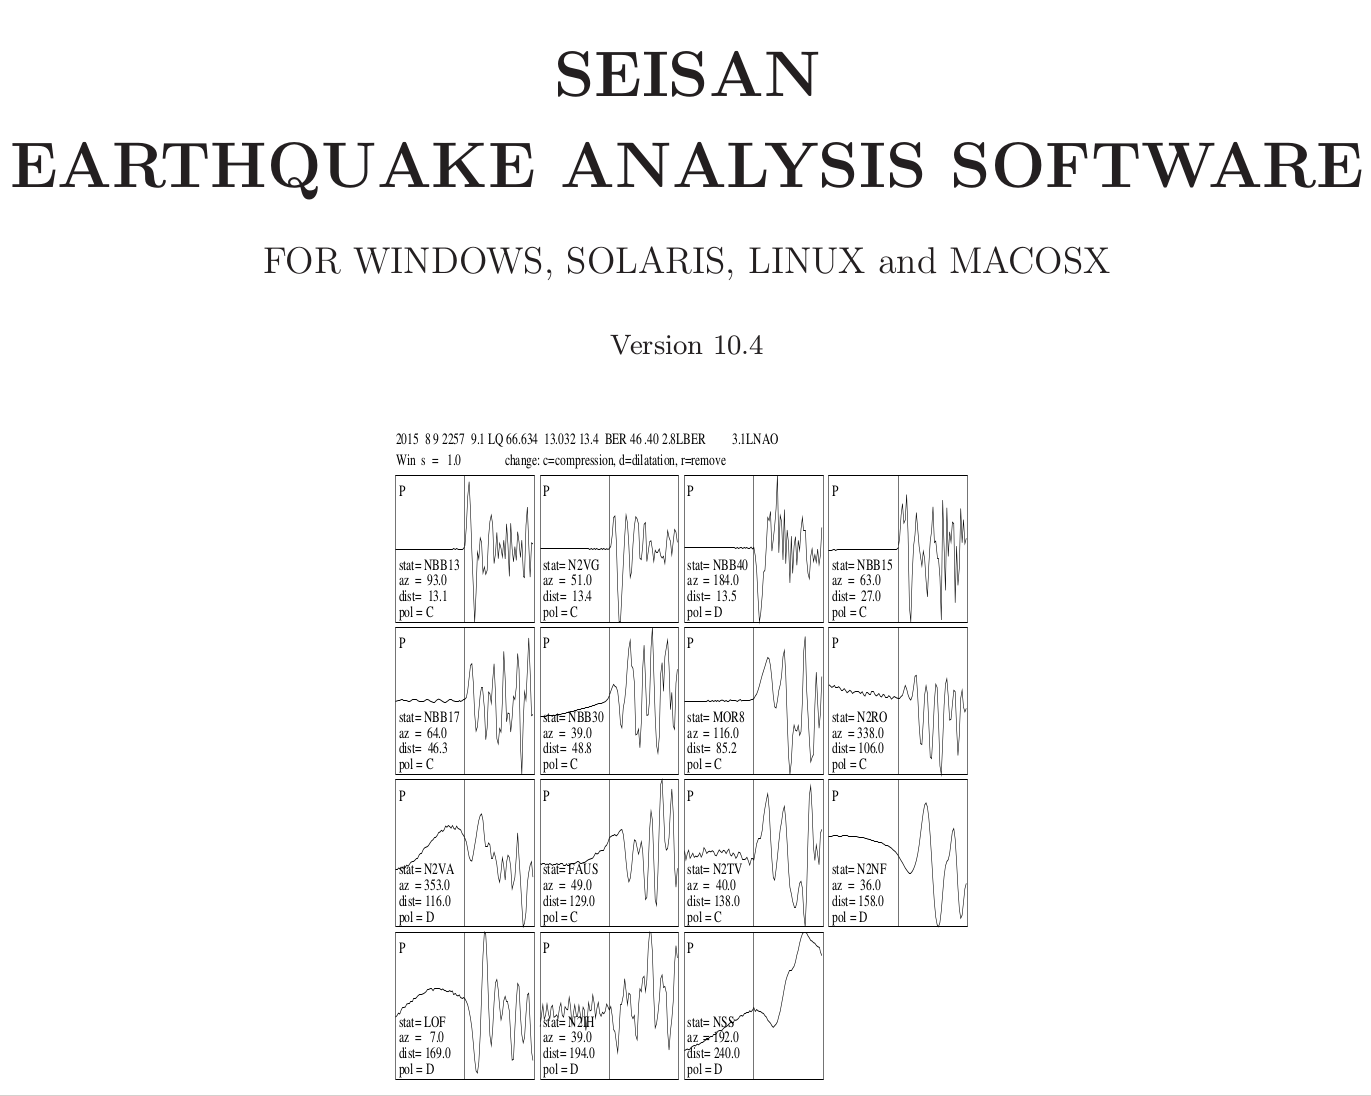
\includegraphics[scale=0.2]{seisan_portada.png}
\end{figure}
\end{frame}
\begin{frame}{SEISAN}
SEISAN (SEISmic ANalysis System) esta constituido por una base de datos de eventos sísmicos y un conjunto de programas que permiten analizar de forma rutinaria los eventos que ocurren tanto local como globalmente. 
\begin{itemize}
\item Permite almacenar y consultar los eventos sísmicos en un formato estándar.\\
\pause
\item Permite el procesamiento de catálogos extensos de eventos sísmicos.\\
\pause
\item Procesamiento básico (rutina) y avanzado en sismología.
\pause
\item Es un software multiplataforma (Linux, MacOS, Windows).\\
\pause
\end{itemize}
\end{frame}
\begin{frame}{SEISAN}
Donde se encuentrar SEISAN
\begin{itemize}
\item \url{http://seisan.info/}
\item \url{https://www.youtube.com/watch?v=KJH3ktGL_K0}
\item Localmente en {\tt /bd/seismo/INF/}
\end{itemize}
\end{frame}

\section{Estructura de SEISAN}
\subsection{Estructura básica}
\begin{frame}{Estructura de SEISAN}
\begin{figure}
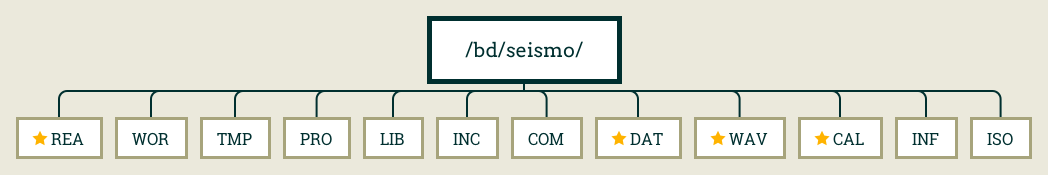
\includegraphics[scale=0.28]{estructura_seisan_1.png}
\end{figure}
\end{frame}

\begin{frame}{Estructura de SEISAN}
\begin{figure}
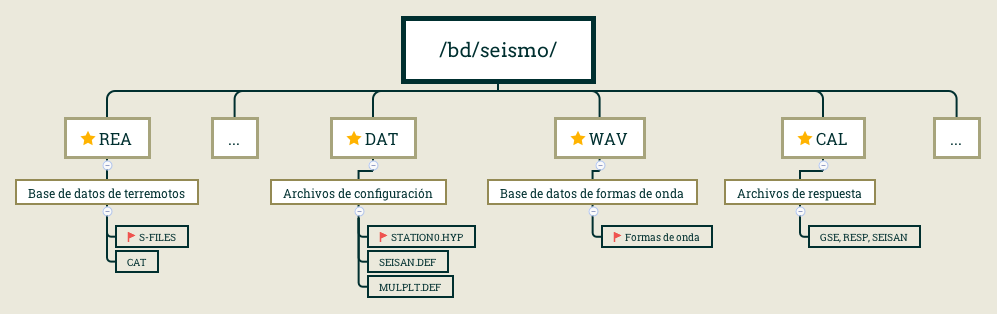
\includegraphics[scale=0.28]{estructura_seisan2.png}
\end{figure}
\end{frame}

\begin{frame}{Estructura de SEISAN}
\begin{figure}
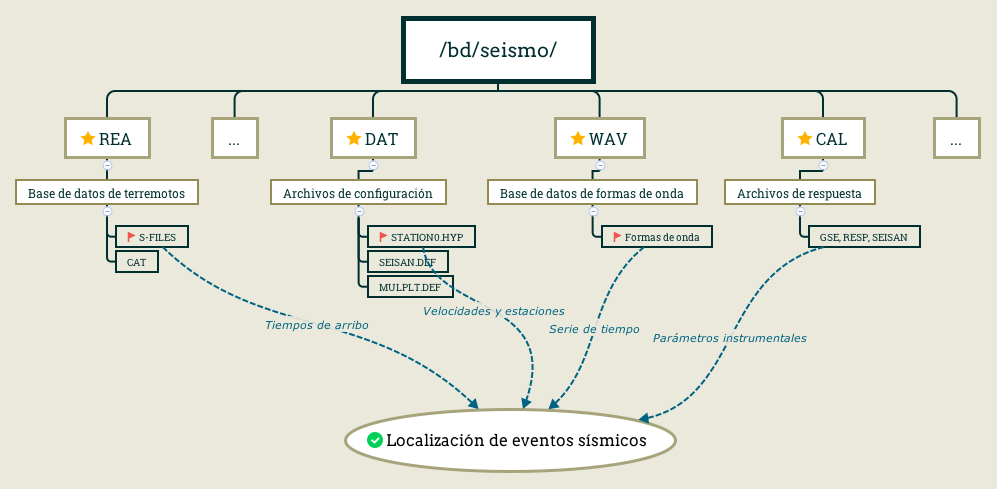
\includegraphics[scale=0.28]{estructura_seisan3.png}
\end{figure}
\end{frame}

\subsection{WAV}
\begin{frame}{WAV}
WAV es la base de datos de formas de onda. Las formas de onda son series de tiempo de los registros de la velocidad del suelo. Estas formas de onda se almacenan en formato digital para facilitar su intercambio y procesamiento.\\

\begin{figure}
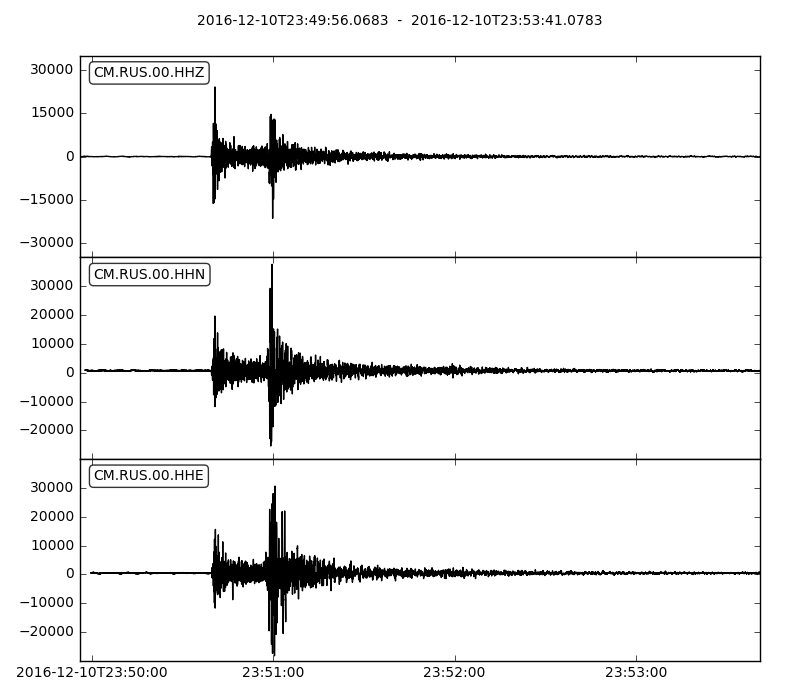
\includegraphics[scale=0.2]{sismo_RUS.png}
\caption{Sismograma digital de un evento sísmico.}
\end{figure}
\end{frame}

\begin{frame}{Formatos de sismogramas digitales}
Existen diferentes formatos para almacenar formas de onda:
\begin{itemize}
\item Formato SEISAN.\\
\pause
\item Formato SAC (Seismic Analysis Code).\\
\pause
\item Passcal.\\
\pause
\item GCF (Guralp Compressed Format).\\
\pause
\item Standard for the Exchange of Earthquake Data (SEED).\\
\pause 
\end{itemize}
Estos formatos almacenan la información en canales simples y volúmenes multicanal junto con los metadatos de cada serie de tiempo. 
\end{frame}

\begin{frame}
Los metadatos básicos de una serie de tiempo en formato miniSEED son:
\begin{center}
{\tt       network: CM\\
         station: RUS\\
        location: 00\\
         channel: HHZ\\
       starttime: 2009-08-24T00:20:03.000000Z\\
         endtime: 2009-08-24T00:20:32.990000Z\\
   sampling\_rate: 100.0\\
              delta: 0.01\\
            npts: 3000\\}
\end{center}
\end{frame}


\subsubsection{{\tt mulplt}}
\begin{frame}{WAV: comando {\tt mulplt}}
\begin{figure}
\includegraphics[scale=0.15]{TRAZA.png}
\end{figure}
Las archivos de formas de onda tienen nombres como {\tt 2014-06-25-0726-38M.COL\_\_\_256}.
\end{frame}


\begin{frame}{WAV: comando {\tt dirf}}
El comando {\tt dirf} crea una lista numerada de archivos:\\
{\small \tt 
 \$ dirf *.COL*\\
 \#  1  2014-06-25-0726-38M.COL\_\_\_ 256 \\                                        
 \#  2  2016-09-25-0500-00M.COL\_\_\_ 327 \\                                        
 \#  3  2016-09-26-1633-25M.COL\_\_\_ 336 \\
}
\end{frame}



\subsection{REA}
\begin{frame}[fragile]{REA}
Es la base de datos de soluciones de hipocentros de eventos sísmicos. Para ingresar:\\
\begin{minted}{bash}
$cd /bd/seismo/REA
\end{minted}
\begin{minted}{bash}
$re
\end{minted}
\end{frame}

\begin{frame}{REA}
La base de datos REA está compuesta por archivos de texto plano conocidos cómo S-files:\\
\begin{center}
\begin{figure}
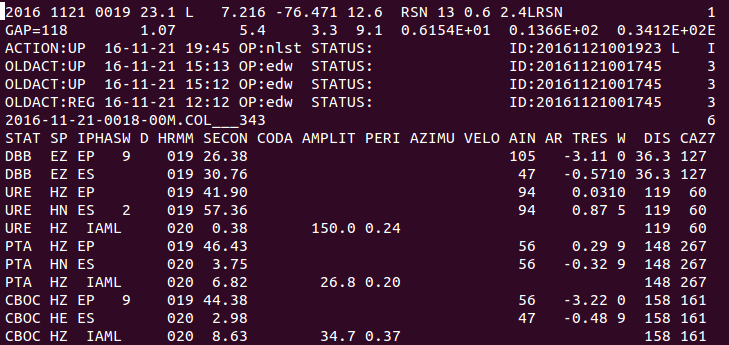
\includegraphics[scale=0.3]{sfile.png}
\end{figure}
\end{center}
El nombre típico del s-file es de la forma {\tt 21-0019-23L.S201611}.
\end{frame}

\begin{frame}[fragile]{REA: comando {\tt eev}}
Con el fin de acceder a la base de datos se utiliza el comando {\tt eev}. Es un entorno que permite gestionar facilmente la base de datos de s-files.\\
{\scriptsize \tt
\$eev 20161121 BDRSN\\
2016 11 Reading events from base OPERA  3127\\ 
\# 2238 21 Nov 2016 00:19 23  L   7.216 -76.471 12.6    0.6 2.4LRSN   13  ?\\
\# 2235 21 Nov 2016 00:49 14  L   6.759 -73.132145.1    0.3 1.7LRSN    6  ?\\
}
\end{frame}

\begin{frame}{REA: comando {\tt eev}}
Los comandos básicos del entorno {\tt eev} son: 
\begin{table}
\begin{tabular}{|c|c|}
\hline 
{\bf Comando}  & {\bf Descripción} \\ 
\hline 
Ir al siguiente S-file & \keys{\return} \\ 
\hline 
Ir al S-file anterior & b \keys{\return} \\ 
\hline 
Editar evento & e \keys{\return} \\ 
\hline 
Comentar evento & com \keys{\return} \\ 
\hline
Localizar evento & l \keys{\return} \\ 
\hline
Actualizar evento & u \keys{\return} \\ 
\hline
Ver forma de onda & po \keys{\return} \\ 
\hline
Ver nombre del S-file & tt \keys{\return} \\ 
\hline
Ver nombre de forma de onda & w \keys{\return} \\ 
\hline
\end{tabular} 
\end{table}
\end{frame}



%\begin{frame}{Antes de comenzar...}
%Existen distintos tipos y clasificaciones para lenguajes de programación:
%\begin{itemize}
%\item Lenguajes de bajo nivel (``assembler``) y lenguajes de alto nivel (C++, C, Java, Perl, Bash, \textbf{Python}).
%\pause
%\item Lenguajes con diferente {\it paradigma} de programación: orientados a objetos, imperativos, funcionales.
%\pause
%\item Lenguajes compilados (C, C++, Fortran) y lenguajes interpretados (Bash, \textbf{Python}).
%\end{itemize}
%\end{frame}
%
%\begin{frame}
%\begin{figure}
%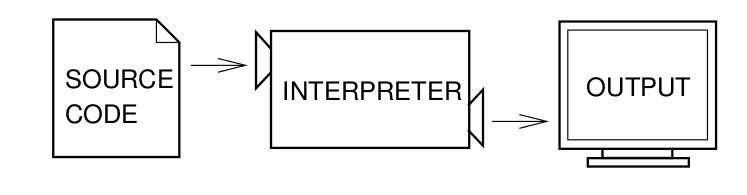
\includegraphics[scale=0.3]{interpretado.png}
%\caption{Esquema de lenguaje interpretado}
%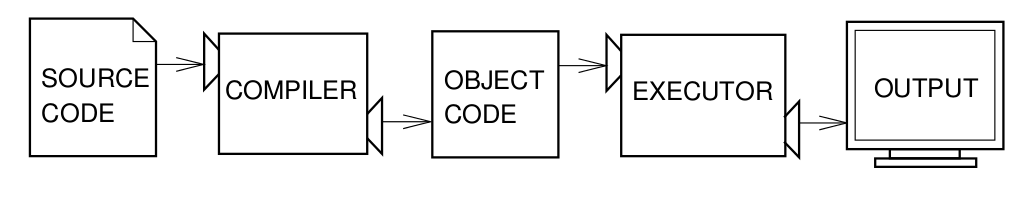
\includegraphics[scale=0.3]{compilado.png}
%\caption{Esquema de lenguaje compilado}
%\end{figure}
%\end{frame}
%
%\subsection{¿Qué es Python?}
%\begin{frame}
%\begin{center}
%\begin{huge}
%¿QUÉ ES PYTHON?
%\end{huge}
%\end{center}
%\end{frame}
%
%\begin{frame}{¿Qué es python?}
%Python es un lenguaje de programación diseñado por Guido Van Rossum. Su primera versión se publicó en 1991 y actualmente cuenta con dos versiones estables 2.7 y 3.5
%\begin{figure}
%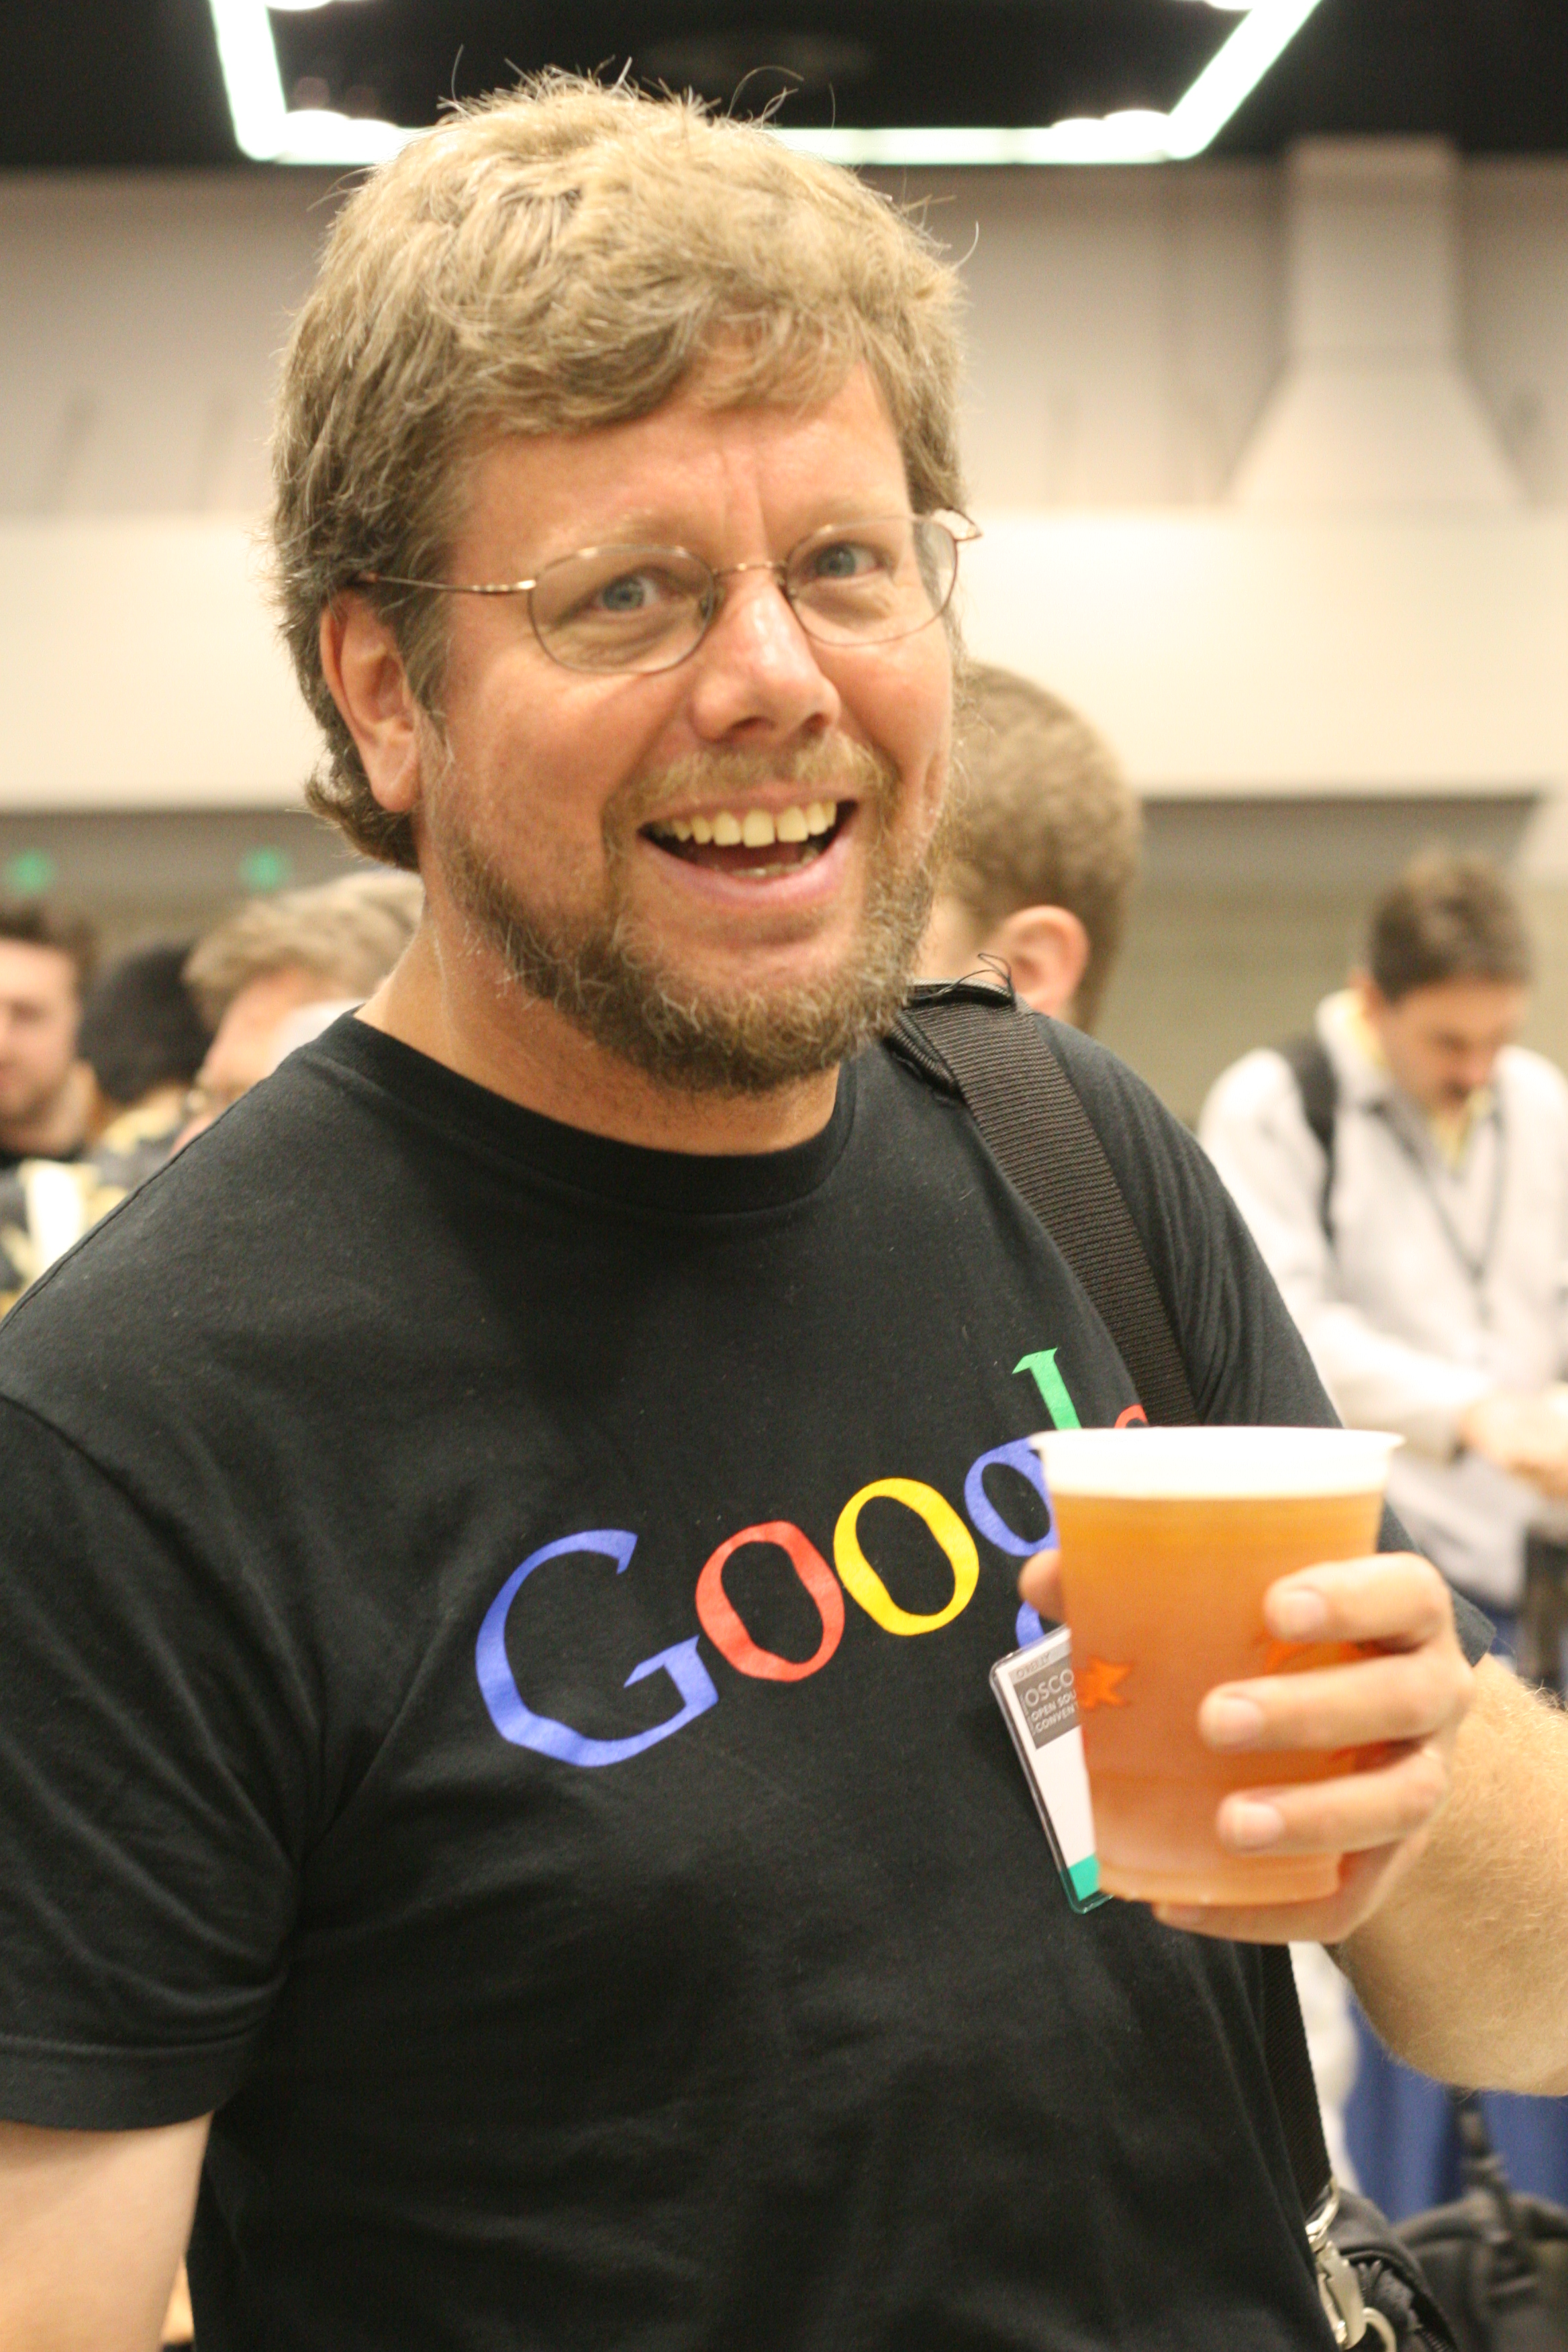
\includegraphics[scale=0.03]{guido.jpg}
%\caption{Benevolente Dictador Vitalicio}
%
\includegraphics[scale=0.2]{python-logo.png}
%\end{figure}
%\end{frame}
%
%\begin{frame}{Características}
%\begin{itemize}
%\item \textbf{Python} es un lenguaje de programación de alto nivel interpretado.
%\pause
%\item \textbf{Python} es portable. Los programas se pueden ejecutar en distintas plataformas sin (muchas) modificaciones.
%\pause
%\item \textbf{Python} es multiparadigma. Permite programación orientada a objetos y programación imperativa.
%\pause
%\item Posee licencia de código abierto compatible con la licencia general de GNU.
%\end{itemize}
%\end{frame}
%
%\begin{frame}{Instalación}
%Existen multiples formas de instalar \textbf{Python}. En nuestro caso utilizaremos la siguiente:
%\begin{center}
%\begin{figure}
%
\includegraphics[scale=0.5]{anaconda.png}\\
%\url{https://www.continuum.io/downloads}
%\end{figure}
%\end{center}
%\end{frame}
%
%
%\section{Variables, expresiones y declaraciones}
%
%\subsection{Valores y Tipos}
%\begin{frame}[fragile]{Valores y Tipos}
%\textbf{Python} utiliza diferentes tipos de valores para la ejecución de programas: cadenas de caracteres, enteros, punto flotante entre otros.
%\begin{minted}{python}
%>>> type('Hola, Mundo')
%<type 'str'>
%>>> type(17)
%<type 'int'>
%>>> type(3.2)
%<type 'float'>
%\end{minted}
%\end{frame}
%
%\subsection{Variables}
%\begin{frame}[fragile]{Variables}
%Una variable es un nombre que se refiere a un valor:
%\begin{minted}{python}
%>>>nombre = 'Guido'
%>>>print 'Mi nombre es '+nombre
%Mi nombre es Guido
%\end{minted} 
%\end{frame}
%
%\begin{frame}{Variables}
%Mejor vamos a la terminal...
%\begin{figure}
%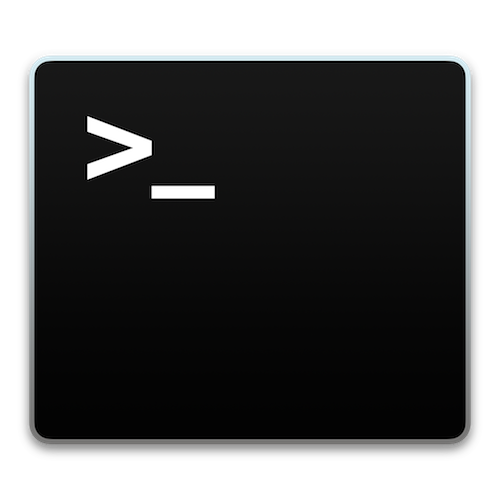
\includegraphics[scale=0.5]{terminal.png}
%\end{figure}
%\end{frame}
%\begin{frame}{Palabras clave de Python}
%Python tiene algunas palabras reservadas:\\
%\begin{center}
%{\tt and   \tab    del   \tab    from   \tab   not  \tab     while\\
%as   \tab     elif  \tab    global  \tab  or   \tab     with\\
%assert  \tab  else   \tab   if    \tab    pass  \tab    yield\\
%break   \tab  except  \tab  import  \tab  print\\
%class  \tab   exec   \tab   in    \tab    raise\\
%continue \tab finally \tab  is    \tab    return \\
%def   \tab    for   \tab    lambda  \tab  try\\
%}
%\end{center}
%\end{frame}
%
%\subsection{Listas}
%\begin{frame}{Listas}
%Una lista es una secuencia de valores ordenados
%\begin{figure}
%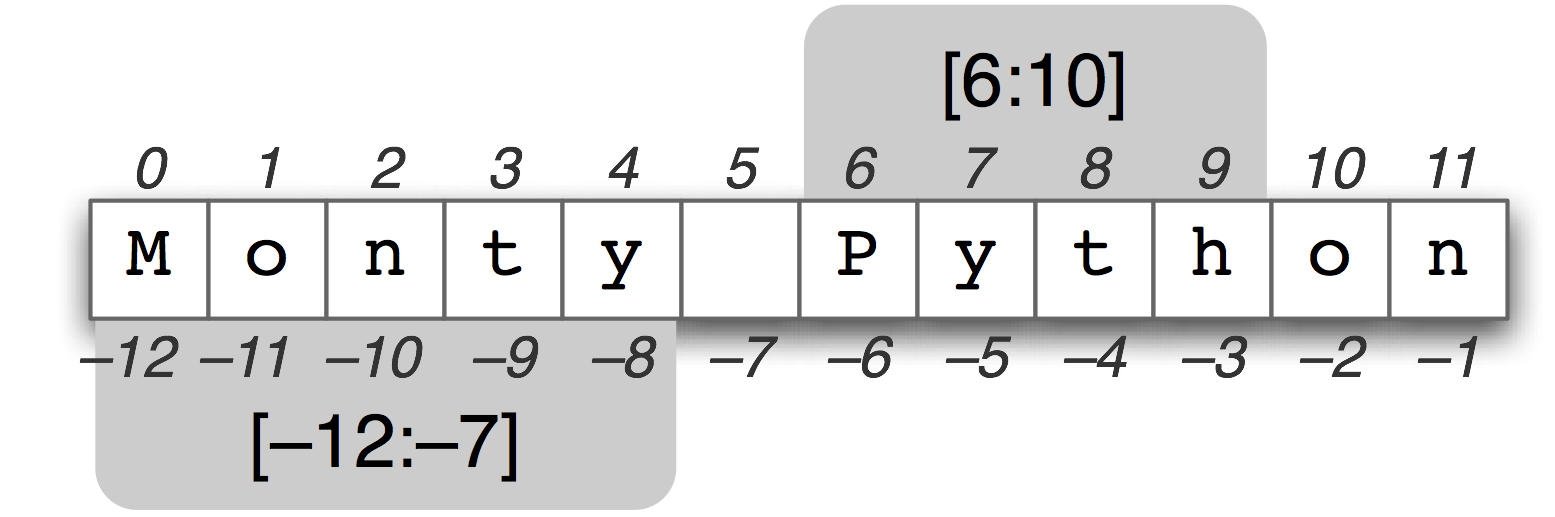
\includegraphics[scale=0.5]{lista.png}
%\end{figure}
%\end{frame}
%
%
%\section{Funciones Integradas}
%
%\begin{frame}{Funciones integradas (Built-in Functions)}
%\begin{itemize}
%\item Una {\bf función} es una secuencia de declaraciones que realizan un cálculo identificadas con un nombre.\\
%\item Un {\bf módulo } es un archivo que contiene un conjunto de funciones relacionadas.
%\item Algunas funciones integradas son: {\tt int(), float(), str(), type(), print, dir(), abs(), len(), open(), range()}
%\end{itemize}
%\end{frame}
%
%\begin{frame}{Funciones integradas}
%Volvamos  a la terminal
%\begin{figure}
%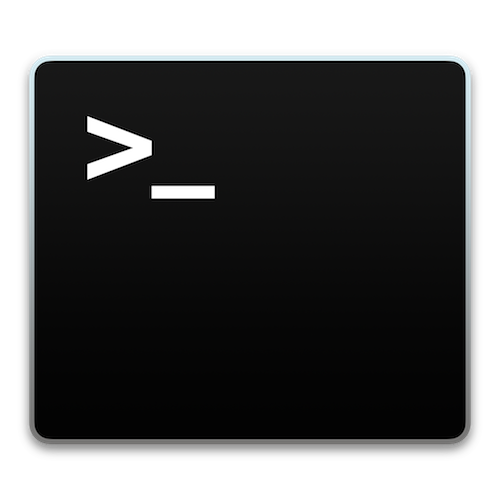
\includegraphics[scale=0.5]{terminal.png}
%\end{figure}
%\end{frame}
%
%\section{Condicionales y Ciclos}
%%\definecolor{bg}{rgb}{0.95,0.95,0.95}
%
%%\defverbatim[colored]\exampleCode{
%
%%}
%\subsection{Condicionales}
%\begin{frame}[fragile]{Condicionales}
%La ejecución condicional permite cambiar el comportamiento de un programa dependiendo del valor de una expresión. Ej:
%%\exampleCode
%\begin{minted}{python}
%if x > 0:
%    print 'x es positivo'
%elif:
%    print 'x es 0 o negativo'
%\end{minted}
%\end{frame}
%
%\subsection{Ciclos}
%\begin{frame}[fragile]{Ciclos}
%\begin{columns}
%\begin{column}{0.5\linewidth}
%\begin{exampleblock}{Ciclo While}
%\begin{minted}{python}
%n=10
%while n > 0:
%    print n
%    n = n-1
%print 'Stop!'
%\end{minted}
%\end{exampleblock}
%\end{column}
%\pause
%\begin{column}{0.5\linewidth}
%\begin{exampleblock}{Ciclo for}
%\begin{minted}{python}
%s = 'Hola Mundo!!'
%for i in range(len(s)):
%    print l[i]
%\end{minted}
%\end{exampleblock}
%\end{column}
%\end{columns}
%\end{frame}
\end{document}